\documentclass[12pt]{article}
\usepackage{times}
\usepackage[hungarian,british]{babel}
\usepackage{url}
\usepackage{latexsym}
\usepackage[utf8]{inputenc}
\usepackage[hidelinks]{hyperref}
\usepackage{color}
\usepackage[dvipsnames]{xcolor}
\definecolor{OliveGreen}{rgb}{0,0.6,0}
\usepackage{graphicx}
\usepackage{booktabs,amsmath,multicol,bm}
\usepackage{breakcites}
\usepackage{float}
\usepackage{tikz-qtree}
\usepackage[nottoc]{tocbibind}
\setcounter{secnumdepth}{3}
\newcommand{\tab}[1]{\hspace{.2\textwidth}\rlap{#1}}
\usepackage[top=2.5cm, bottom=4cm, left=2.5cm, right=2.5cm]{geometry}
\usepackage{array}
\newcolumntype{L}[1]{>{\raggedright\let\newline\\\arraybackslash\hspace{0pt}}m{#1}}


\begin{document}

\section{Cross-entropy loss}
A general encoder-decoder architecture is trained one input-output pair at a time. First the encoder encodes the input, then the decoder starts generating the output. At each step the decoder is conditioned on the generated word (word embedding) in the previous step. During training the generated word at each step is replaced by the word in the target sequence. 

An example target could be the sequence \textit{I love apples}, with a vocabulary consisting of only these words. Firstly, the decoder's softmax layer generates probabilities over the vocabulary for the first word, and the loss function is the cross-entropy between the predicted probabilities and the one-hot vector of target probabilities:
\begin{equation}
L(\bm y,\bm t) = -\bm y \log \bm t
\end{equation}
Where \(\bm y\) is the vector containing the predicted probabilities from the softmax, and \(\bm t\) is the target one-hot vector, which is 1 for the current target word, and 0 for any other word in the vocabulary. This loss is backpropagated, and then the token \textit{I} is fed into the next step of the decoder, and the whole process repeats itself.

\section{Proposed method}
I define a new loss function, where instead of the one-hot vector a distribution over all words is used, according to the training set. Suppose that we have a training set, where for the same input there are 3 different targets (all padded to the same length):
\begin{itemize}
	\item Thanks \textless pad\textgreater \textless pad\textgreater
	\item Thanks and you
	\item Not so good
\end{itemize}

Thus, there are in total 7 words in our vocabulary. The training procedure is as follows. The decoder predicts probabilities over the vocabulary the same way as before in the first step. However, instead of the one-hot vector, the following vector is used for the cross entropy loss:
\(\bm t=[1/3, 2/3, 0, 0, 0, 0, 0]\) corresponding to the words: \([Not, Thanks, <pad>, and, you, so, good]\).

The cross-entropy loss is calculated in the same way. After backpropagation, before getting to the second step, we have to choose a word which will be fed into the decoder at the next step. I propose, to use roulette-wheel selection over the target probabilities. Thus, there is a 1/3 chance to select \textit{Not}, and a 2/3 chance to select \textit{Thanks}. After this the selected word's embedding is fed into the next state of the decoder. If the word \textit{Not} was chosen then the following target vector is used to calculate the loss in the second step: \(\bm t=[0, 0, 0, 0, 0, 1, 0]\), since according to the training set, if the first word was \textit{Not}, the only possible next word is \textit{so}. If the word \textit{Thanks} was chosen then the target vector is: \(\bm t=[0, 0, 1/2, 1/2, 0, 0, 0]\), similarly. The loss is backpropagated and again a word is chosen based on the target probabilities to feed into the next state of the decoder. The process continues until we get to the end of the sequence. A visualization is given below.
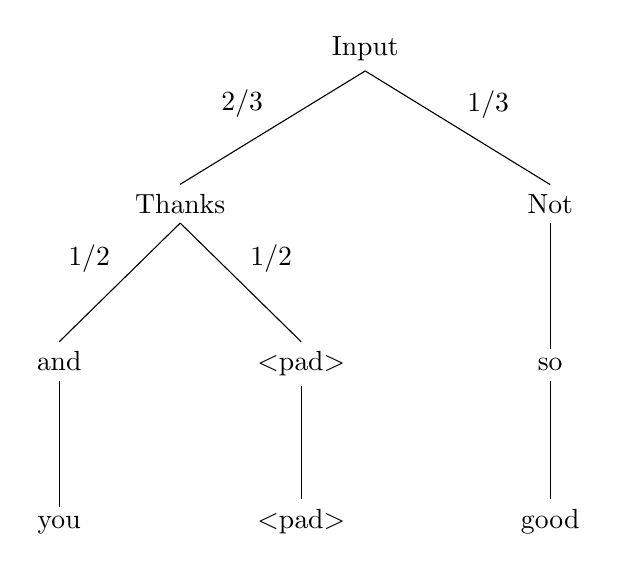
\begin{tikzpicture}[level distance=2cm, sibling distance=2cm]

\Tree 
[.{Input}
	\edge node[auto=right] {2/3};
	[.{Thanks}
		\edge node[auto=right] {1/2};
		[.{and}
			[.you ] ]
		\edge node[auto=left] {1/2};
		[.{\textless pad\textgreater}
			[.{\textless pad\textgreater} ] ]
	]
	\edge node[auto=left] {1/3};
	[.{Not} 
		[.{so}
			[.{good} ] ]
	]
]
\end{tikzpicture}

	
\end{document}
